\section{手法と実験}

\subsection{データ分析}

データの分析例を図\ref{fig:scatter}に示す.

\begin{figure}[H]
  \centering
  \begin{tikzpicture}[scale=1.0]
  % 座標軸
  \draw[->] (-0.5,0) -- (5,0) node[right] {$x$};
  \draw[->] (0,-0.5) -- (0,4) node[above] {$y$};
  
  % グリッド
  \draw[gray!30, thin] (0,0) grid (4.5,3.5);
  
  % データポイント
  \fill[blue] (1,1) circle (3pt);
  \fill[blue] (2,1.8) circle (3pt);
  \fill[blue] (3,2.5) circle (3pt);
  \fill[blue] (4,3.2) circle (3pt);
  
  % 近似直線
  \draw[red, thick, dashed] (0.5,0.5) -- (4.5,3.5);
  
  % ラベル
  \node[blue] at (4.2,3.5) {データ};
  \node[red] at (3.5,2.5) {近似線};
\end{tikzpicture}

  \caption{データの散布と近似線}
  \label{fig:scatter}
\end{figure}

\subsection{関数の比較}

複数の関数の比較を図\ref{fig:functions}に示す.

\begin{figure}[H]
  \centering
  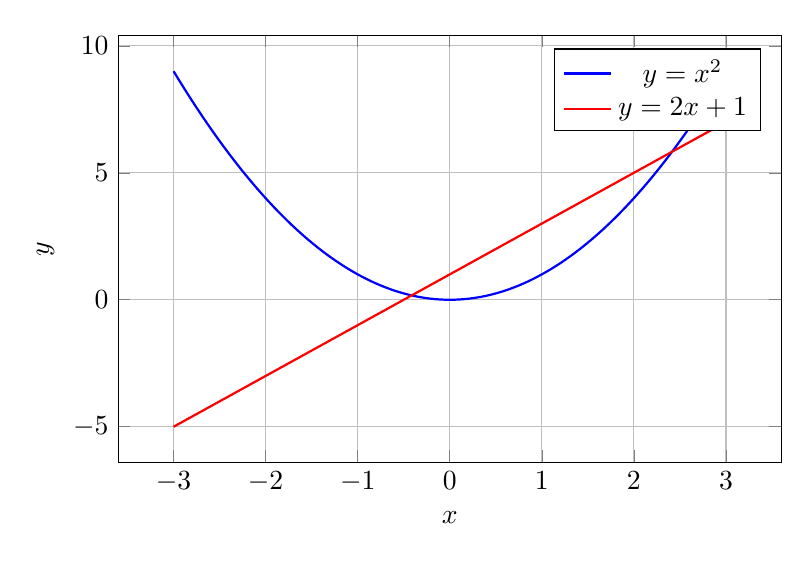
\begin{tikzpicture}
  \begin{axis}[
    xlabel={$x$},
    ylabel={$y$},
    grid=major,
    width=10cm,
    height=7cm,
    legend pos=north east
  ]
  \addplot[blue, thick, domain=-3:3, samples=100] {x^2};
  \addplot[red, thick, domain=-3:3, samples=100] {2*x+1};
  \legend{$y=x^2$, $y=2x+1$}
  \end{axis}
\end{tikzpicture}

  \caption{関数のプロット例}
  \label{fig:functions}
\end{figure}


